\documentclass[12pt]{article}

% This first part of the file is called the PREAMBLE. It includes
% customizations and command definitions. The preamble is everything
% between \documentclass and \begin{document}.

\usepackage[margin=1in]{geometry}  % set the margins to 1in on all sides
\usepackage{graphicx}              % to include figures
\usepackage{amsmath}               % great math stuff
\usepackage{amsfonts}              % for blackboard bold, etc
\usepackage{amsthm}                % better theorem environments
\usepackage{amssymb} 
\usepackage{mathptmx}
\usepackage{enumerate}
\usepackage{listings}
\usepackage{xcolor}
\usepackage{forest}
\usepackage{tabularx}  

% various theorems, numbered by section

\newtheorem{thm}{Theorem}[section]
\newtheorem{lem}[thm]{Lemma}
\newtheorem{prop}[thm]{Proposition}
\newtheorem{cor}[thm]{Corollary}
\newtheorem{conj}[thm]{Conjecture}
\newtheorem{mydef}[thm]{Definition}
\lstset{
	basicstyle          =   \sffamily,          
	keywordstyle        =   \bfseries,          
	commentstyle        =   \rmfamily\itshape,  
	stringstyle         =   \ttfamily,  
	flexiblecolumns,                
	numbers             =   left,   
	showspaces          =   false,  
	numberstyle         =   \fontsize{5}{skip},    
	showstringspaces    =   false,
	captionpos          =   t,      
	frame               =   lrtb,   
}

\lstdefinestyle{cpp}{
	language        =   cpp, 
	basicstyle      =   \fontsize{5}{skip},
	numberstyle     =   \fontsize{5}{skip},
	keywordstyle    =   \color{blue},
	keywordstyle    =   [2] \color{teal},
	stringstyle     =   \color{magenta},
	commentstyle    =   \color{red}\ttfamily,
	breaklines      =   true,   
	columns         =   fixed,  
	basewidth       =   0.5em,
}
\begin{document}


\title{ CSE 102 Spring 2021\\
	Quiz Reflection 4}

\author{Jaden Liu \\ 
University of California at Santa Cruz\\
Santa Cruz, CA 95064 USA }

\maketitle


\section{Quiz 4} 

\begin{proof}[Solution for 1]
	b): (s,w) will be the shortest path from s to w, however, it will never determine any other shortest path during this step.
\end{proof}
\begin{proof}[Solution for 4]
	Here is an counter example.\\
	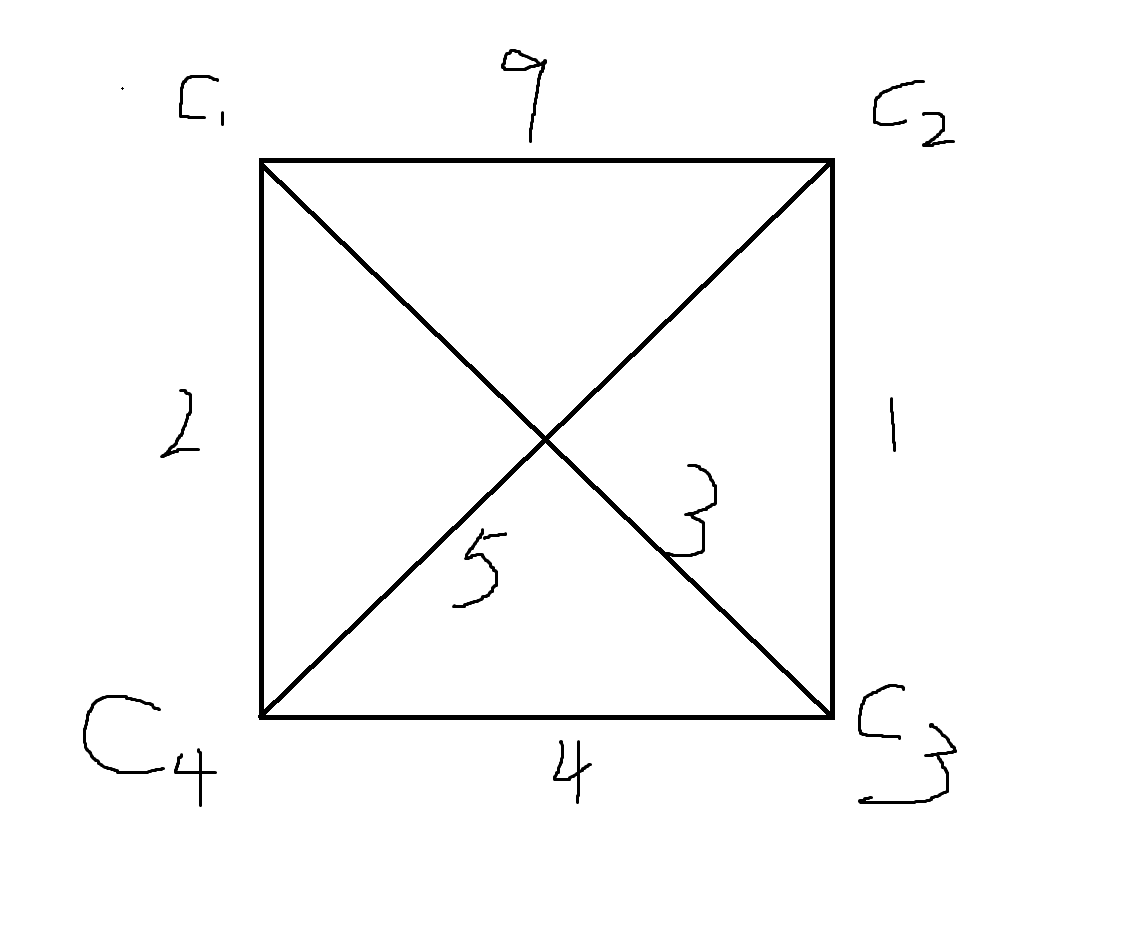
\includegraphics[scale=0.25]{4.png}\\
	By greedy algorithm: $c_1\rightarrow c_4\rightarrow c_3 \rightarrow c_2 \rightarrow c_1 =2+4+1+9=16$.\\
	While the optimal solution is: $c_1\rightarrow c_4\rightarrow c_2 \rightarrow c_3\rightarrow c_1=2+5+1+3=11$.\\
\end{proof}
\begin{proof}[Solution for 5]
	I didn't notice we only need to prove the denomination 1 case, so I only need to provide why $g_1$ and $n_1$ is from 0 to 5. The whole proof would be:\\
	Let c=\{$c_1=1,c_2=5,c_3=10,c_4=5^2$\}\\
	Suppose we have X=\{$x_1,x_2,x_3,x_4$\} be the optimal solution.\\
	Let g=\{$g_1,g_2,g_3,g_4$\} be the solution to our greedy algorithm.\\
	Now we need to prove that $\sum_{i=1}^{4}x_ic_i=\sum_{i=1}^{4}g_ic_i$:\\
	$x_1+5x_2+10x_3+25x_4 = g_1+5g_2+10g_3+25g_4$\\
	reduing the equation by mod 5 yielding $x_1\equiv g_1$(mod 5).\\
	$0\le g_1 <5$ because greedy algorithm will choose larger denomination if $g_1$ is larger than or equal than 5 in last selection.\\
	$0\le n_1 <5$ because optimal solution will reduce the amount of $n_1$. However, if $n_1$ is larger than 5, it could not be the optimal solution.\\
	Thus $n_1=g_1$ mod 5, and $n_1=g_1$.
\end{proof}
\begin{proof}[Solution for 6]
	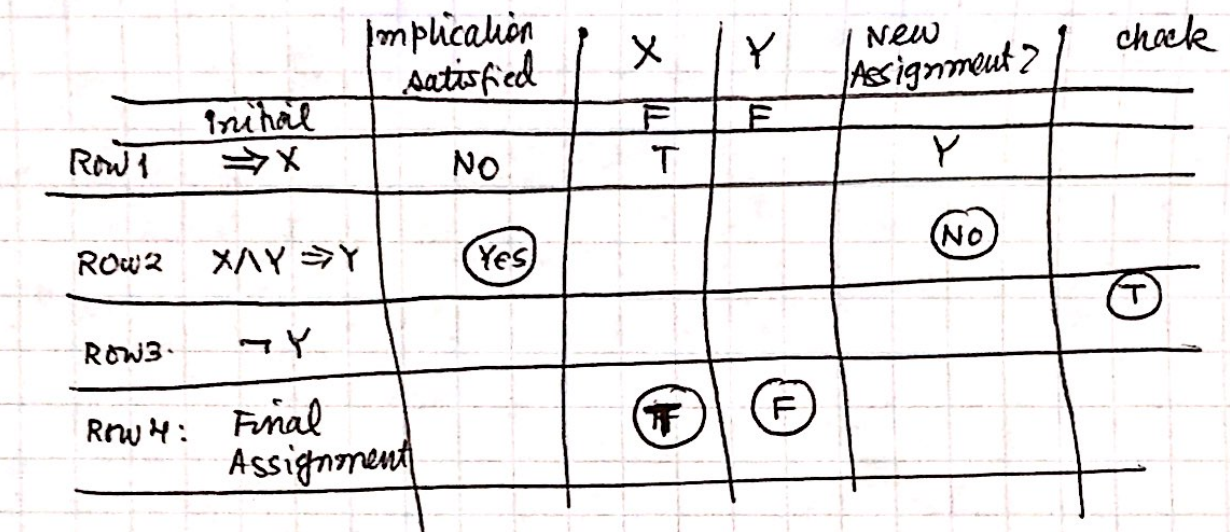
\includegraphics[scale=0.25]{6.png}\\
	After $X$ change to true from false, "$X$ and $Y$" will maintain false. "false$\rightarrow$false" statement will maintain true. And all the following result will change as well. Y would stay F, check would be true.
\end{proof}
\bigskip



\end{document}
